\section{Results}
\label{sec:results}

All results are on the PTB-XL test fold (fold~10, \nTestRecords{} records), and all models receive the same corrupted
test data for each condition. Values for LG-EDL and the corruption-trained ResNet are mean\,$\pm$\,standard deviation
over three seeds; the other variants were trained once. For random lead removal, each value is first averaged over
the three draws of that condition.

% ---------------------------------------------------------------------------------------------------------------
\subsection{Clean Test Performance}
\label{sec:res-clean}

\begin{table}[t]
\centering
\caption{Clean test performance. Mean\,$\pm$\,standard deviation over three seeds where available, otherwise one
run. ECE: expected calibration error over all $N\times5$ binary predictions (15 bins). All models except LG-EDL are
temperature-scaled on the validation fold.}
\label{tab:clean}
\begin{adjustbox}{max width=\columnwidth}% generated by make_numbers.py from results/table1.csv
\begin{tabular}{@{}lcccc@{}}
\toprule
Model & Seeds & Macro-AUROC & Macro-F1 & ECE \\
\midrule
LG-EDL & 3 & 0.903\,$\pm$\,0.001 & 0.715\,$\pm$\,0.004 & 0.032\,$\pm$\,0.011 \\
LG-soft & 1 & 0.906 & 0.715 & 0.014 \\
LG-hard & 1 & 0.907 & 0.726 & 0.012 \\
ResNet + lead attention & 1 & 0.909 & 0.726 & 0.014 \\
ResNet, corruption-trained & 3 & 0.903\,$\pm$\,0.000 & 0.706\,$\pm$\,0.005 & 0.015\,$\pm$\,0.003 \\
ResNet, clean-trained & 1 & 0.896 & 0.693 & 0.011 \\
Patch Transformer & 1 & 0.885 & 0.680 & 0.015 \\
MLP & 1 & 0.722 & 0.486 & 0.054 \\
XGBoost & 1 & 0.823 & 0.598 & 0.013 \\
\bottomrule
\end{tabular}
\end{adjustbox}
\end{table}

On complete recordings the six convolutional models, the two ResNets and the four lead-attention variants, range
from \aucResCleanClean{} (ResNet, clean-trained) to \aucResAttnClean{} (un-gated lead attention, one run)
(Table~\ref{tab:clean}). LG-EDL reaches \aucLgEdlCleanPM{} and the corruption-trained ResNet \aucResDropCleanPM; their
paired difference is \bootCleanDiff{} (95\% CI \bootCleanCI). The patch Transformer (\aucTransClean), XGBoost
(\aucXgbClean) and the MLP (\aucMlpClean) are weaker. All scores are below the published PTB-XL benchmark for the
same task at 100\,Hz, where the best single model reached \litBestSingleAuc{} and an ensemble \litEnsembleAuc{}
\cite{strodthoff2021benchmark}; with no hyperparameter tuning and at most 15 epochs, absolute performance is not
the subject of this study.

For every model, hypertrophy is the hardest class (LG-EDL \pcLgEdlHyp, corruption-trained ResNet \pcResDropHyp) and
NORM the easiest (\pcLgEdlNorm{} and \pcResDropNorm). LG-EDL has an ECE of \eceLgEdlCleanPM, against
\eceResDropCleanPM{} for the corruption-trained ResNet and between \eceResCleanClean{} and \eceResAttnClean{} for the
other ResNet and attention variants. Because only LG-EDL is not temperature-scaled, this difference does not show
that the evidential head itself is less calibrated.

% ---------------------------------------------------------------------------------------------------------------
\subsection{Training With Simulated Lead Failure}
\label{sec:res-dropout}

\begin{figure*}[t]
\centering
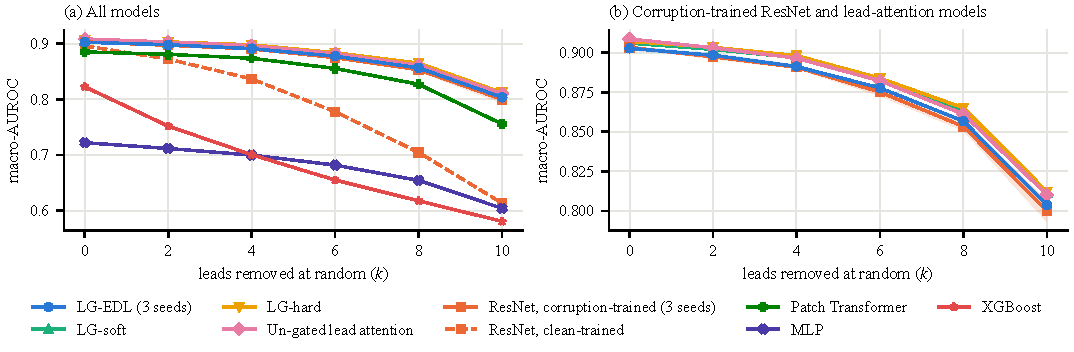
\includegraphics[width=\textwidth]{fig_random.pdf}
\caption{Macro-AUROC on the test fold as $k$ randomly chosen leads are removed (three draws per $k$). (a) All models.
(b) The five corruption-trained ResNet and lead-attention models, which overlap in (a). Bands: standard deviation
over three seeds where available.}
\label{fig:random}
\end{figure*}

\begin{table}[t]
\centering
\caption{Macro-AUROC with $k$ leads removed at random (mean over three draws, then over seeds).}
\label{tab:random}
\begin{adjustbox}{max width=\columnwidth}% generated by make_numbers.py from results/random_loss.csv (mean over 3 draws, then over seeds)
\begin{tabular}{@{}lcccccc@{}}
\toprule
& \multicolumn{6}{c}{Leads removed at random ($k$)} \\
\cmidrule(l){2-7}
Model & 0 & 2 & 4 & 6 & 8 & 10 \\
\midrule
LG-EDL & 0.903 & 0.898 & 0.891 & 0.878 & 0.857 & 0.804 \\
LG-soft & 0.906 & 0.902 & 0.897 & 0.883 & 0.863 & 0.811 \\
LG-hard & 0.907 & 0.903 & 0.898 & 0.884 & 0.865 & 0.812 \\
ResNet + lead attention & 0.909 & 0.903 & 0.897 & 0.882 & 0.861 & 0.810 \\
ResNet, corruption-trained & 0.903 & 0.897 & 0.891 & 0.875 & 0.853 & 0.800 \\
ResNet, clean-trained & 0.896 & 0.872 & 0.837 & 0.778 & 0.705 & 0.613 \\
Patch Transformer & 0.885 & 0.881 & 0.874 & 0.856 & 0.827 & 0.756 \\
MLP & 0.722 & 0.712 & 0.700 & 0.682 & 0.654 & 0.604 \\
XGBoost & 0.823 & 0.752 & 0.700 & 0.655 & 0.617 & 0.581 \\
\bottomrule
\end{tabular}
\end{adjustbox}
\end{table}

The training data separate the models more than the architecture does (Fig.~\ref{fig:random},
Table~\ref{tab:random}). The ResNet trained on clean recordings falls from \aucResCleanKZero{} with all leads to
\aucResCleanKTen{} with ten leads removed. The same architecture trained with simulated failures falls from
\aucResDropKZero{} to \aucResDropKTenPM, so at $k=10$ the two training regimes differ by \gainDropKTen. The
corruption-trained ResNet loses nothing on clean data (\aucResDropClean{} against \aucResCleanClean). The
clean-trained ResNet is a single run, but the gap at $k=10$ is more than twenty times the seed standard deviation of
the corruption-trained ResNet. The difference also holds at the decision level: at $k=10$, macro-F1 is
\foneResCleanKTen{} for the clean-trained and \foneResDropKTen{} for the corruption-trained ResNet.

With corruption training, the ResNet and the four attention variants lie close together at $k=10$: LG-EDL
\aucLgEdlKTenPM, LG-soft \aucLgSoftKTen, LG-hard \aucLgHardKTen, un-gated attention \aucResAttnKTen{} and ResNet
\aucResDropKTen. The attention variants span \ablRangeKTen, and the best is \gapAttnResKTen{} above the ResNet. The
patch Transformer, which mixes all leads within each token, degrades more (\aucTransKTen). XGBoost, trained on clean
records and given removed leads as missing features, falls from \aucXgbKZero{} to \aucXgbKTen, and the
corruption-trained MLP from \aucMlpKZero{} to \aucMlpKTen.

\begin{table}[t]
\centering
\caption{Macro-AUROC with a lead group removed, or with an artifact on six random leads (EMG at 10\,dB, baseline
wander, clipping).}
\label{tab:group}
\begin{adjustbox}{max width=\columnwidth}% generated by make_numbers.py from results/group_loss.csv and results/artifact.csv
\begin{tabular}{@{}lcccccc@{}}
\toprule
& \multicolumn{3}{c}{Lead group removed} & \multicolumn{3}{c}{Artifact on 6 leads} \\
\cmidrule(lr){2-4}\cmidrule(l){5-7}
Model & V1--V6 & Limb & V1--V3 & EMG & Wander & Clip \\
\midrule
LG-EDL & 0.871 & 0.869 & 0.882 & 0.898 & 0.891 & 0.889 \\
LG-soft & 0.877 & 0.870 & 0.887 & 0.900 & 0.895 & 0.893 \\
LG-hard & 0.878 & 0.869 & 0.888 & 0.895 & 0.894 & 0.890 \\
ResNet + lead attention & 0.876 & 0.874 & 0.888 & 0.904 & 0.903 & 0.893 \\
ResNet, corruption-trained & 0.873 & 0.868 & 0.882 & 0.903 & 0.899 & 0.894 \\
ResNet, clean-trained & 0.747 & 0.809 & 0.851 & 0.896 & 0.844 & 0.877 \\
Patch Transformer & 0.853 & 0.845 & 0.864 & 0.885 & 0.875 & 0.880 \\
MLP & 0.661 & 0.679 & 0.669 & 0.721 & 0.684 & 0.723 \\
XGBoost & 0.666 & 0.734 & 0.743 & 0.814 & 0.749 & 0.727 \\
\bottomrule
\end{tabular}
\end{adjustbox}
\end{table}

The same pattern holds when a lead group is removed (Table~\ref{tab:group}). The precordial leads V1--V6 run across
the chest from the right sternal border to the left axillary line and record the heart in the horizontal plane
\cite{kligfield2007recommendations}; they are the main view of the anterior wall and carry much of the ST-segment,
T-wave and QRS-amplitude information. Without them, the clean-trained ResNet falls to \aucResCleanPrec, against
\aucResDropPrec{} after corruption training. The loss is not limited to infarction: for the clean-trained ResNet, the
AUROC for MI falls from \pcResCleanMi{} to \pcResCleanMiPrec, that for ST/T change from \pcResCleanSttc{} to
\pcResCleanSttcPrec, and that for NORM from \pcResCleanNorm{} to \pcResCleanNormPrec, whereas the corruption-trained
ResNet keeps \pcResDropMiPrec, \pcResDropSttcPrec{} and \pcResDropNormPrec. With baseline wander on six leads, the two
training regimes reach \aucResCleanWanderSix{} and \aucResDropWanderSix.

% ---------------------------------------------------------------------------------------------------------------
\subsection{Quality Gating}
\label{sec:res-gating}

\begin{table}[t]
\centering
\caption{Lead-attention variants (all corruption-trained): macro-AUROC on clean data, with $k=6$ and $k=10$ leads
removed at random and without V1--V6, and clean ECE. Three of the four variants are single runs.}
\label{tab:ablation}
\begin{adjustbox}{max width=\columnwidth}% generated by make_numbers.py from results/table2.csv
\begin{tabular}{@{}lcccccc@{}}
\toprule
Variant & Seeds & Clean & $k{=}6$ & $k{=}10$ & V1--V6 & ECE \\
\midrule
ResNet + lead attention & 1 & 0.909 & 0.882 & 0.810 & 0.876 & 0.014 \\
LG-hard & 1 & 0.907 & 0.884 & 0.812 & 0.878 & 0.012 \\
LG-soft & 1 & 0.906 & 0.883 & 0.811 & 0.877 & 0.014 \\
LG-EDL & 3 & 0.903 $\pm$ 0.001 & 0.878 $\pm$ 0.000 & 0.804 $\pm$ 0.002 & 0.871 $\pm$ 0.002 & 0.032 $\pm$ 0.011 \\
\bottomrule
\end{tabular}
\end{adjustbox}
\end{table}

The four attention variants share the per-lead encoder and the attention code and differ only in whether attention
and pooling are weighted by the estimated quality and in the output head (Table~\ref{tab:ablation}). Their clean
macro-AUROC spans \ablRangeClean{} and their macro-AUROC at $k=10$ spans \ablRangeKTen. The un-gated variant has the
highest clean score (\aucResAttnClean) and is never the lowest of the four under random or group lead loss. Three of
the variants are single runs and were not compared statistically; for scale, the largest seed standard deviation of
LG-EDL under random lead loss is \seedStdLgEdlMaxLoss. The ablation therefore shows no benefit of gating larger than
about 0.01 in this setting and cannot exclude a smaller one.

The paired bootstrap of LG-EDL against the corruption-trained ResNet covers the clean condition, 15 random-removal
draws, three group removals and nine artifact conditions (Appendix, Table~\ref{tab:bootstrap}). None of the
\bootNRows{} intervals lies entirely above zero. The intervals of \bootNSigNeg{} conditions lie entirely below zero,
all of them artifacts: baseline wander on two, four and six leads (\bootWanderTwoDiff, \bootWanderFourDiff,
\bootWanderSixDiff) and EMG on six leads (\bootEmgSixDiff). The intervals are uncorrected and the conditions share
test records; with \bootNRows{} comparisons at the 5\% level, about one would exclude zero by chance if the two
models were equivalent. That all four are negative and three are wander conditions suggests a systematic effect,
which we treat as tentative.

A possible reason, not tested here, is that the assessor was trained to label leads with strong wander as
unreliable, following our severity rule, so the gated models down-weight such leads although their QRS complexes
remain readable. Under wander on six leads, the three gated variants (\aucLgHardWanderSix, \aucLgSoftWanderSix,
\aucLgEdlWanderSix) score below both the un-gated model (\aucResAttnWanderSix) and the ResNet (\aucResDropWanderSix).

Two observations limit what the ablation can test. Replacing the estimated quality by the true quality changes
macro-AUROC by at most \oracleMaxAbsDiff{} for any gated run and condition, so the accuracy of the quality estimate
is not the limiting factor. And the simulated failures are easy to detect: removed leads are zero or constant, the
assessor scores untouched clean leads at \sqaMeanQClean{} on average, and its agreement with the reliability label is
at least \sqaGate{} for every failure type outside the borderline band. Its scores are therefore close to binary,
which is why hard and soft gating behave almost identically, and the soft weighting is barely exercised.

% ---------------------------------------------------------------------------------------------------------------
\subsection{Evidential Uncertainty and Abstention}
\label{sec:res-edl}

\begin{figure*}[t]
\centering
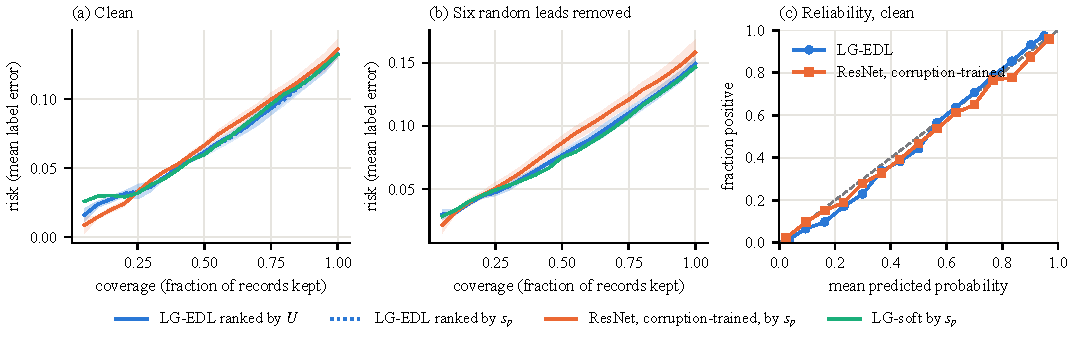
\includegraphics[width=\textwidth]{fig_riskcov.pdf}
\caption{(a, b) Risk--coverage curves: records are kept in order of increasing uncertainty, and risk is the mean
fraction of the five labels predicted wrongly at the validation-tuned thresholds; $s_p$ is the probability-based
score of Section~\ref{sec:setup-metrics}. (c) Reliability diagram on the clean test fold (LG-EDL not
temperature-scaled).}
\label{fig:riskcov}
\end{figure*}

\begin{table}[t]
\centering
\caption{Risk (mean per-record label error) at 50\%, 80\% and 100\% coverage and mean risk over 20 coverage levels
from 5\% to 100\%. $U$: evidential uncertainty; $s_p$: probability-based score.}
\label{tab:selective}
\begin{adjustbox}{max width=\columnwidth}% generated by make_numbers.py from results/risk_coverage.csv
\begin{tabular}{@{}lcccc@{}}
\toprule
Model, score & 50\% & 80\% & 100\% & Mean \\
\midrule
\multicolumn{5}{@{}l}{\emph{Clean}} \\
LG-EDL, $U$ & 0.062 & 0.102 & 0.133 & 0.068 \\
LG-EDL, confidence & 0.061 & 0.100 & 0.133 & 0.068 \\
LG-soft, confidence & 0.060 & 0.104 & 0.132 & 0.069 \\
ResNet + attn., conf. & 0.056 & 0.095 & 0.126 & 0.066 \\
ResNet (corr.), conf. & 0.066 & 0.106 & 0.136 & 0.070 \\
\midrule
\multicolumn{5}{@{}l}{\emph{6 random leads removed}} \\
LG-EDL, $U$ & 0.077 & 0.117 & 0.149 & 0.083 \\
LG-EDL, confidence & 0.077 & 0.117 & 0.149 & 0.083 \\
LG-soft, confidence & 0.075 & 0.116 & 0.147 & 0.081 \\
ResNet + attn., conf. & 0.074 & 0.115 & 0.148 & 0.082 \\
ResNet (corr.), conf. & 0.087 & 0.129 & 0.159 & 0.090 \\
\bottomrule
\end{tabular}
\end{adjustbox}
\end{table}

If the evidential head added useful uncertainty, ranking records by $U$ would give a lower risk at a given coverage
than ranking them by $s_p$ from the same model. It does not (Table~\ref{tab:selective}, Fig.~\ref{fig:riskcov}). On
clean data, LG-EDL ranked by $U$ has a risk of \riskLgEdlUCleanHalf{} at 50\% coverage, against
\riskLgEdlConfCleanHalf{} when ranked by $s_p$, and the mean risk over all coverage levels is \aurcLgEdlUClean{} for
both. With six leads removed the values are again equal (\riskLgEdlUKSixHalf{} and \riskLgEdlConfKSixHalf{} at 50\%
coverage). The lowest clean risk at 50\% coverage belongs to the un-gated attention model ranked by $s_p$
(\riskResAttnConfCleanHalf). These differences were not tested statistically.

\begin{figure*}[t]
\centering
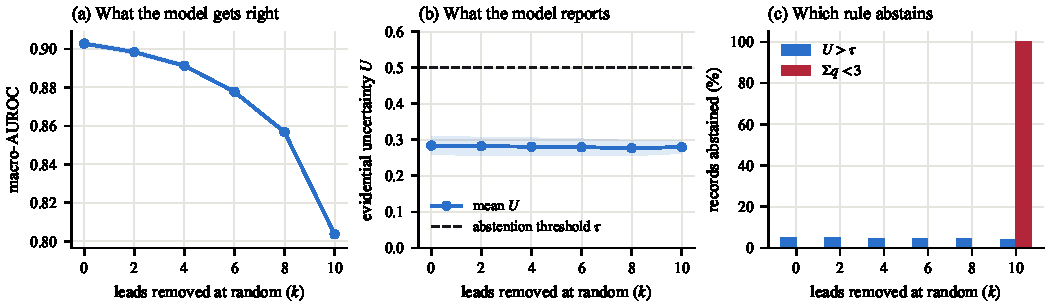
\includegraphics[width=\textwidth]{fig_certainty.pdf}
\caption{LG-EDL as leads are removed at random. (a) Macro-AUROC. (b) Mean evidential uncertainty $U$ and the
abstention threshold $\tau$. (c) Share of records rejected by each abstention rule. Lines: mean over three seeds after
averaging the three draws; bands: standard deviation over seeds.}
\label{fig:certainty}
\end{figure*}

\begin{table}[t]
\centering
\caption{LG-EDL abstention as leads are removed at random (mean over draws, then seeds). $\tau$ is the 95th
percentile of $U$ on the clean validation fold.}
\label{tab:abstain}
\begin{adjustbox}{max width=\columnwidth}% generated by make_numbers.py from results/abstain_rate.csv (LG-EDL, mean over draws then seeds)
\begin{tabular}{@{}cccccc@{}}
\toprule
$k$ & Abstain (\%) & $U{>}\tau$ (\%) & $\Sigma q{<}3$ (\%) & Mean $U$ & Mean $\Sigma q$ \\
\midrule
0 & 5.1 & 5.1 & 0.0 & 0.284 & 11.96 \\
2 & 4.8 & 4.8 & 0.0 & 0.282 & 9.97 \\
4 & 4.5 & 4.5 & 0.0 & 0.281 & 7.98 \\
6 & 4.5 & 4.5 & 0.0 & 0.279 & 5.99 \\
8 & 4.6 & 4.6 & 0.0 & 0.277 & 3.99 \\
10 & 100.0 & 4.0 & 100.0 & 0.279 & 2.00 \\
\bottomrule
\end{tabular}
\end{adjustbox}
\end{table}

$U$ also does not respond to missing leads (Fig.~\ref{fig:certainty}, Table~\ref{tab:abstain}). As $k$ goes from 0 to
10, LG-EDL's macro-AUROC falls from \aucLgEdlKZero{} to \aucLgEdlKTen, while its mean $U$ changes from \meanUKZero{}
to \meanUKTen. The $U$ rule rejects \abstainUKZero\% of test records with all leads present and between
\abstainUKTen\% and \abstainUKTwo\% for every $k$ up to ten, close to the 5\% set on validation data. The lead-count
rule never fires while four or more leads remain (mean $\sum_j q_j$ of \meanQsumKEight{} at $k=8$) and rejects every
record at $k=10$. Under lead loss, abstention beyond the clean-data rate therefore comes only from the lead-count
rule, which for these failures needs neither the evidential head nor a learned quality score.

The flat $U$ is not accompanied by a loss of calibration in LG-EDL's probabilities. Its pooled ECE is
\eceLgEdlKZero{} with all leads, \eceLgEdlKEight{} at $k=8$ and \eceLgEdlKTen{} at $k=10$, against \eceResDropKZero,
\eceResDropKEight{} and \eceResDropKTen{} for the corruption-trained ResNet. We did not record per-condition summaries
of $s_p$, so we cannot say whether the probability-based score rises with $k$.

% ---------------------------------------------------------------------------------------------------------------
\subsection{An Example Record}
\label{sec:res-case}

\begin{figure*}[t]
\centering
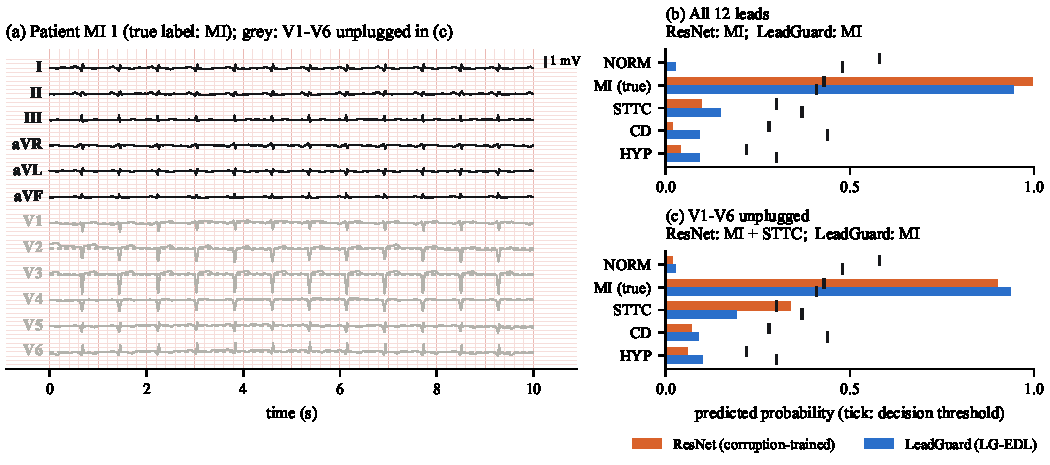
\includegraphics[width=\textwidth]{fig_vignette.pdf}
\caption{One test record before and after V1--V6 are removed. (a) The raw recording; the grey leads are removed in
(c). (b, c) Class probabilities of the corruption-trained ResNet and LG-EDL; ticks mark each model's validation-tuned
decision threshold. The record was selected from records that both models classify correctly with all leads; it
illustrates the behaviour described above and does not show how often it occurs.}
\label{fig:vignette}
\end{figure*}

Fig.~\ref{fig:vignette} shows one test record, \vigPatient, labelled MI only. With all leads both models are
correct; the ResNet gives MI a probability of \vigBaseMiFull{} and LG-EDL \vigLgMiFull. Without V1--V6, the ResNet
still detects MI (\vigBaseMiCut), but its probability for ST/T change rises from \vigBaseStFull{} to \vigBaseStCut,
above its threshold of \vigBaseStThr, so it adds a false label. LG-EDL keeps MI as its only label (\vigLgMiCut), and
its $U$ changes from \vigLgUFull{} to \vigLgUCut. On average neither pattern favours one model
(Section~\ref{sec:res-gating}).
